\documentclass{article}
\usepackage[utf8]{inputenc}

\usepackage[
  colorlinks=true,
  linkcolor=blue,
  citecolor=teal,
  urlcolor=magenta,
  pdfusetitle
]{hyperref}

\usepackage[dvipsnames,svgnames,table]{xcolor}
\usepackage{tikz}
\usepackage{circuitikz}
\usetikzlibrary{arrows, shapes, backgrounds, positioning, calc, arrows.meta}


\usepackage{listings}

\lstdefinelanguage{Dafny}{
  morekeywords = {
    class, datatype, type, iterator,
    bool, nat, int, set, seq,
    function, predicate,
    ghost, var,
    method,
    returns, module, import, in,
    requires, ensures, reads, decreases,
    match, case, false, true, null,
    assert, assume, print, new, if, then, else, while,
    invariant, label, return, calc, forall, exists
  },
  sensitive        = true,
  morecomment      = [l]{//},
  morestring       = [b]",
  literate =
    {:=}{{$:=$}}2 {<=}{{$\le$}}1 {>=}{{$\ge$}}1
    {==>}{{$\Rightarrow$}}2 {<==>}{{$\Leftrightarrow$}}2
    {forall}{{$\forall$}}1 {exists}{{$\exists$}}1 {!=}{{$\neq$}}1,
}
\lstset{
  language        = Dafny,
  basicstyle      = \ttfamily\small,
  keywordstyle    = \color{RoyalBlue}\bfseries,
  commentstyle    = \color{OliveGreen}\itshape,
  stringstyle     = \color{Maroon},
  numbers         = left,
  numberstyle     = \tiny\color{gray},
  frame           = single,
  showstringspaces= false
}

\newcommand{\progname}[1]{\texttt{#1}}

\usepackage[dvipsnames]{xcolor} % Used for the 'plan' environment, at least

\newenvironment{plan}{
  \color{teal}
  \addtolength{\leftskip}{1cm}
}

% There mys be an empty line after the '\newenvironment', otherwise
% LaTeX will report an error.... (S.G.)


\title{Verification of the Quotient Graph construction from the molecule}

\author{
  Yaroslav Rozdobudko
}

\begin{document}

\maketitle

\tableofcontents
\newpage

\section{Introduction}
To make sure that our software works correctly we need to verify it. Usually it is done by testing, but it is not the best solution and in some cases, like critical software it is not sufficient. Quotes by Edsger W. Dijkstra show why\footnote{Quotes by Dijkstra: \url{https://en.wikiquote.org/wiki/Edsger\_W.\_Dijkstra}}:

\begin{quote}
\textit{``Testing shows the presence, not the absence, of bugs.''} --- Edsger W. Dijkstra \cite{buxton1970software}
\end{quote}

\begin{quote}
\textit{``Program testing can be used to show the presence of bugs, but never to show their absence!''} --- Edsger W. Dijkstra \cite{Dijkstra1970}
\end{quote}

It is impossible to came up with all possible test cases, so there might be some inputs that will break the program. But this limitation can be solved by formalizing programs, and introducing proof that program does what it is intended.
Formal verification rigorously proves correctness of program.


The earliest usage of formal methods was by Martin Davis\cite{Davis1957, Davis2002, Mol2025} in his proof of the program for Presburger's algorithm\cite{Presburger1929}.
In 1969 Hoare developed \textit{Hoare triples}\cite{Hoare1969} using Floyd logic\cite{Floyd1967}. \textit{Hoare triple} is of a form $\{P\} C \{Q\}$ where P is the precondition that is required for the program, C is the command after execution of which third part of the triple will be satisfied\footnote{Explained by Hoare: \url{https://www.youtube.com/watch?v=czzp8gMESSY}}. The same paper also provided rules and axioms for work with \textit{Hoare logic}.

Over the years multiple solutions were developed that tried to formalize algorithm. The Boyer-Moore Theorem Prover \textit{Nqthm}\cite{Boyer1992} and \textit{ACL2} proof assistants, automated proof assistant \textit{Isabelle}, languages \textit{Agda}, \textit{Ada/SPARK}, \textit{Dafny}\cite{Leino2010}, \textit{Lean}\footnote{History of program verification: \url{https://www.youtube.com/watch?v=HJkukhoQFzo}}. Formal methods have been used in critical software, hardware design, and also by mathematicians, to help with formal proofs\footnote{The Future of Mathematics \url{https://youtu.be/Dp-mQ3HxgDE?si=hFXAZQEgIvmNDjFb}}.


\section{Dafny}
\subsection{Introduction to Dafny}
Dafny is an imperative language with functional and object oriented features\cite{Leino2010}, and also automated verifier\cite{Herbert2012} based on \textit{dynamic frames}\cite{Kassios2006}.
Dafny verifier will transform source code to the \textit{Boogie}\cite{Barnett2006} language, than from \textit{Boogie} first-order verification conditions are generated and passed to \textit{Z3} SMT solver\cite{deMoura2008} as a query. There is also an option to specify custom SMT solver \texttt{--solver-path} but it is not well documented and there is no support beside \textit{Z3} solver.
\begin{figure}[h]
  \centering
  \resizebox{0.82\textwidth}{!}{
  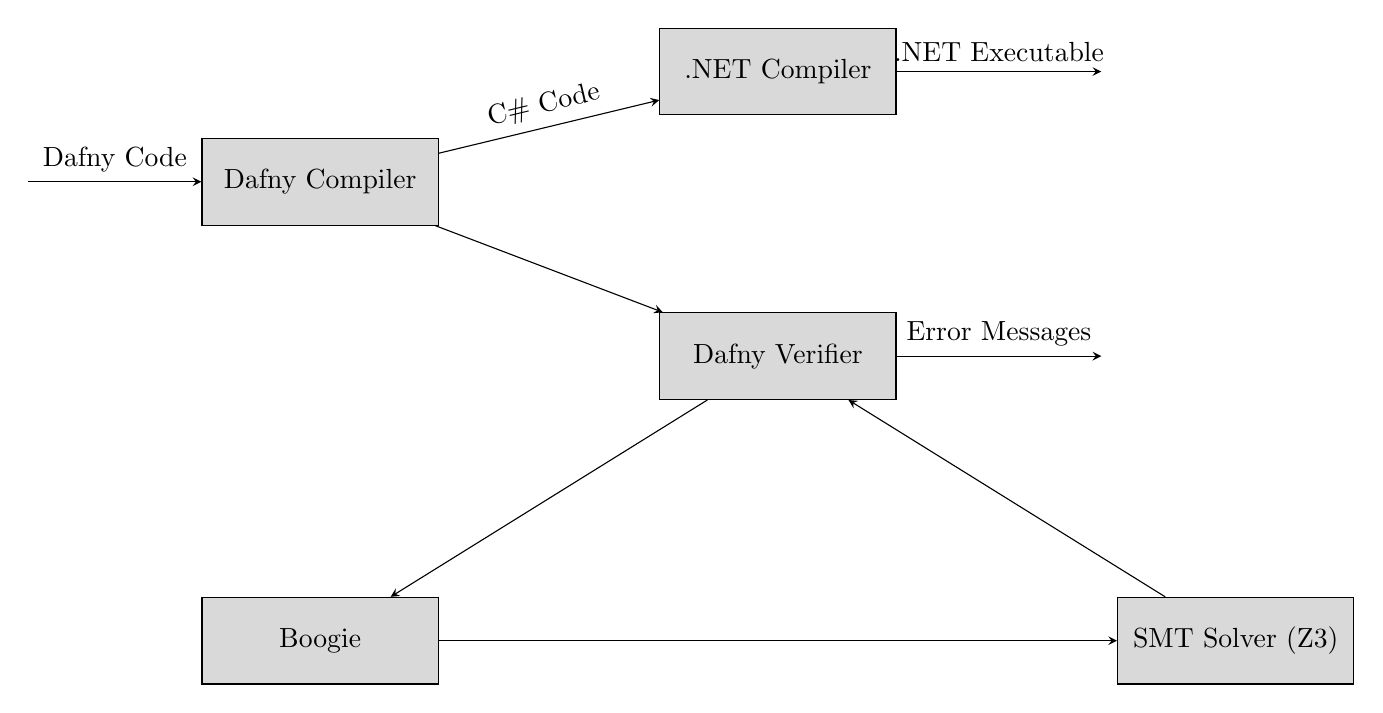
\begin{tikzpicture}[
      >=stealth,
      node distance = 2.5cm and 2.8cm,
      block/.style = {
        draw,
        fill=gray!30,
        minimum width=3cm,
        minimum height=1.1cm,
        align=center
      }
    ]

    \node[block]                       (compiler) {Dafny Compiler};
    \node[block, right=of compiler, yshift=1.4cm] (netcomp) {.NET Compiler};
    \node[block, below=of netcomp]     (verifier) {Dafny Verifier};
    \node[block, below left=of verifier]   (boogie)  {Boogie};
    \node[block, below right=of verifier]  (solver)  {SMT Solver (Z3)};

    \draw[<-] (compiler.west)  -- ++(-2.2cm,0) node[midway,above]{Dafny Code};

    \draw[->] (compiler) -- (netcomp) node[midway,above,sloped]{C\# Code};
    \draw[->] (netcomp.east) -- ++(2.6cm,0) node[midway,above]{.NET Executable};

    \draw[->] (compiler) -- (verifier);

    \draw[->] (verifier.east) -- ++(2.6cm,0) node[midway,above]{Error Messages};

    \draw[->] (verifier) -- (boogie);
    \draw[->] (boogie)   -- (solver);
    \draw[->] (solver)   -- (verifier);

  \end{tikzpicture}
}
  \caption{The Dafny system, figure taken from \cite{Herbert2012}.}
  \label{fig:dafny-system}
\end{figure}

Dafny binaries can be downloaded from the GitHub repository or build from the source code\footnote{Dafny source code: \url{https://github.com/dafny-lang/dafny}}, also can be installed as part of the VS code extension. Dafny \texttt{verify} command takes input Dafny source code with extension \texttt{dfy}, and will output results of the verification. It also supports multiple options like increasing time out for verification or providing more logs about proofs. Separate command can be used to compile Dafny to a number of languages (C\#, Java, Go, JavaScript, C++, Python). There is an also introduction of the Intermediate Representation (IR) which is intermediate language which will allow to compile Dafny to many other languages, and plans to create compiler that will allow to run Dafny code natively\footnote{I heard this news in Dafny video: \url{https://youtu.be/OdTiTiuUMto?si=EuyKXzHr36UTAHCF}}.
It is also possible to translate to \textit{Boogie} code using \texttt{-print} command and run it with the \textit{Boogie}. Even the simplest Dafny program in \textit{Boogie} will contain several thousand lines, because Dafny includes all the specifications needed for the language itself.

\begin{lstlisting}[language=Dafny,caption={Dafny Triple method},label={lst:triple}]
method Triple(x: int) returns (r: int) {
    var y := 2 * x;
    r := x + y;
    assert r == 3 * x;
}
\end{lstlisting}

\begin{lstlisting}[language=Dafny,caption={Boogie Triple method, part of the code translated from Dafny to Boogie},label={lst:boogietriple}]
...
implementation {:smt_option "smt.arith.solver", "2"}
               {:verboseName "Triple (correctness)"}
               Impl$$_module.__default.Triple(x#0: int)
               returns (r#0: int, $_reverifyPost: bool)
{
  var $_ModifiesFrame: [ref,Field]bool;
  var y#0: int;

    // AddMethodImpl: Triple, Impl$$_module.__default.Triple
    $_ModifiesFrame := (lambda $o: ref, $f: Field :: 
      $o != null && $Unbox(read($Heap, $o, alloc)): 
      bool ==> false);
    $_reverifyPost := false;
    // ----- assignment statement ----- Triple.dfy(2,11)
    assume true;
    assume true;
    y#0 := Mul(LitInt(2), x#0);
    // ----- assignment statement ----- Triple.dfy(3,7)
    assume true;
    assume true;
    r#0 := x#0 + y#0;
    // ----- assert statement ----- Triple.dfy(4,4)
    assume true;
    assert {:id "id2"} r#0 == Mul(LitInt(3), x#0);
}
...
\end{lstlisting}

\subsection{How proof works}
Dafny program stored in a text file with extension \texttt{dfy}. We can separate program in the modules with \texttt{module} keyword, and import it in another module. There are multiple built in types: \texttt{bool}, \texttt{int}, \texttt{nat}, etc. In addition to regular operators boolean type supports equivalence (if and only if) \texttt{<===>} and implication \texttt{===>} operators. Dafny numerical types do not have upper bound, since it is supposed to represent mathematical numbers (practically it will of course will be limited by the computer hardware). There are collection types: sets, sequences, maps etc. Dafny supports \textit{quantifiers}, universal \texttt{forall}
\verb|forall x :: P(x)|
which is the same as $\forall{x}: P(x)$, for all x P holds, and existential quantifier \texttt{exists}
\verb|exists x :: P(x)|
which is the same as $\exists{x}: P(x)$, there exists x for whom P holds.

Maps and sets support comprehensions, which can be used to create new maps and sets. Similar to mathematical notation $\{f(x) | R(x)\}$, comprehension
\verb|set x | R :: f(x)| will define the set of all elements $f(x)$ such that $R$ holds. For example we can define a set of squares of integers from 0 to 9 with:
\begin{lstlisting}[language=Dafny,caption={Set comprehension},label={lst:comprehension}]
set x | 0 <= x < 10 :: x * x
\end{lstlisting}

In Dafny \textbf{methods} can take variable number of in parameters and return variable number of out parameters. Methods can be used in statements. Functions can be used in expressions, can take variable number of in parameters but return only one type. We can create \textit{proof obligations} using \textbf{assert} statement, or by specifying \textit{preconditions} using \textbf{requires} keyword and \textit{postconditions} using \textbf{ensures} keyword. Dafny tries to prove \textit{proof obligations} automatically.
We can define \textbf{datatypes} to represent data structures, they do not change state, and can be defined recursively.

To verify that program is correct we need to confirm all the specifications that we used to annotate the program are correct, essentially we make sure that programs adheres to the contract that we specified. By default Dafny will try to verify \textit{proof obligations} automatically, but if it can't it we need to provide additional steps to confirm that \textit{proof obligation} holds. There are multiple ways to prove in Dafny\footnote{Different ways to prove: \url{https://leino.science/papers/krml276.html}}: \textit{lemma}, \textit{assert/assert by}, \textit{calc}. \textit{Assert} statement verifies that a logical preposition is true. Results of the \textit{assert} can be used to prove other \textit{proof obligations}. It is possible to add additional proof steps to \textit{assert} with \textit{by}. \textit{Calc} statements uses \textit{program-oriented calculations} (poC) \cite{Leino2014} and allows us to use list of related expressions, to provide intermediate steps for a proof.

\begin{lstlisting}[language=Dafny,caption={Calc statement, taken from\cite{Leino2023} },label={lst:calc}]
calc {
5 * (x + 3);
== // distribute multiplication over addition
5 * x + 5 * 3;
== // use the arithmetic fact that 5 * 3 == 15
5 * x + 15;
}
\end{lstlisting}

We can reuse program proofs by combining them into \textit{lemmas}, and treat them as an auxiliary theorems that we can use in the proofs, it supports preconditions and postconditions and is a \textit{ghost} method. All the mentioned \textit{proof} tools like \textit{assert} and \textit{calc} are \textit{ghost} constructs, this means that they are not present when we compile Dafny program into an executable program. We can define \textit{ghost} variables or methods ourselves using \texttt{ghost} keyword.

Dafny supports \textit{for} and \textit{while} loops. \textit{While} loop specification consist of \textit{quard} and \textit{invariant}. \textit{Guard} specifies until what state loop should continue, \textit{invariant} restricts states where loop can operate. \textit{Guard} checked before each iteration, \textit{invariant} is checked before loop starts, and after each execution of the loop. By the end of the execution loop will reach state where the \textit{Guard} is false and \textit{invariant} still holds. To prove termination, loops support \textit{decreases} statement.

\begin{lstlisting}[language=Dafny,caption={While loop },label={lst:whileloop}]
method m(){
  var i := 10;
  while 0 < i
    invariant 0 <= i
    decreases i
  {
    i := i - 1;
  }
}
\end{lstlisting}

Here we will check if \textit{invariant} holds, and our \textit{guard} is true, and loop will be executed until $i$ reaches $0$, at this state, \textit{guard} is false but invariant still holds. If we change our invariant to:

\begin{lstlisting}[language=Dafny,caption={Incorrect invariant},label={lst:incorrectloop}]
invariant 2 <= i
\end{lstlisting}

We will get an error:

\begin{lstlisting}[language=Dafny,caption={Error on loop invariant},label={lst:looperror}]
 Related message: loop invariant violation
  |
4 |     invariant 2 <= i
  |
\end{lstlisting}

This is because we cannot guaranty that loop \textit{invariant} holds, since i will be $0$ by the end of the loop execution.


\section{Problem}
\label{sec:description}
It is important to reconstruct molecule from the \textit{asymmetric unit} (AU) preserving stoichiometric ratios. To handle this task program \textit{cif\_molecule}\cite{Grazulis2015} were developed as part of \textit{cod-tools} package.

\begin{tikzpicture}[>=latex]
    \node at ( 0,  0.5) {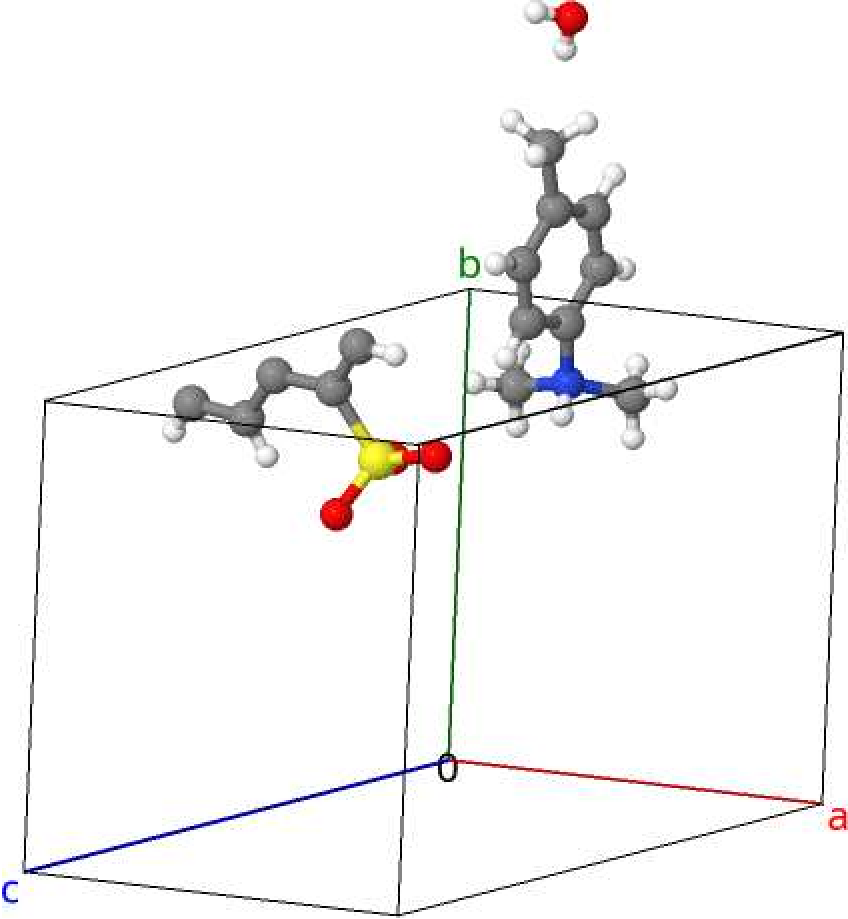
\includegraphics[scale=0.20]{pictures/2231955-crystal}};
    \node at ( 0, -2) {\small\itshape Asymmetric unit};

    \draw[->, ultra thick, rounded corners] ( 2,0) -- (5,0);
    \node at (4,1) {\small\texttt{cif\_molecule}};

    \node at (7, 0) {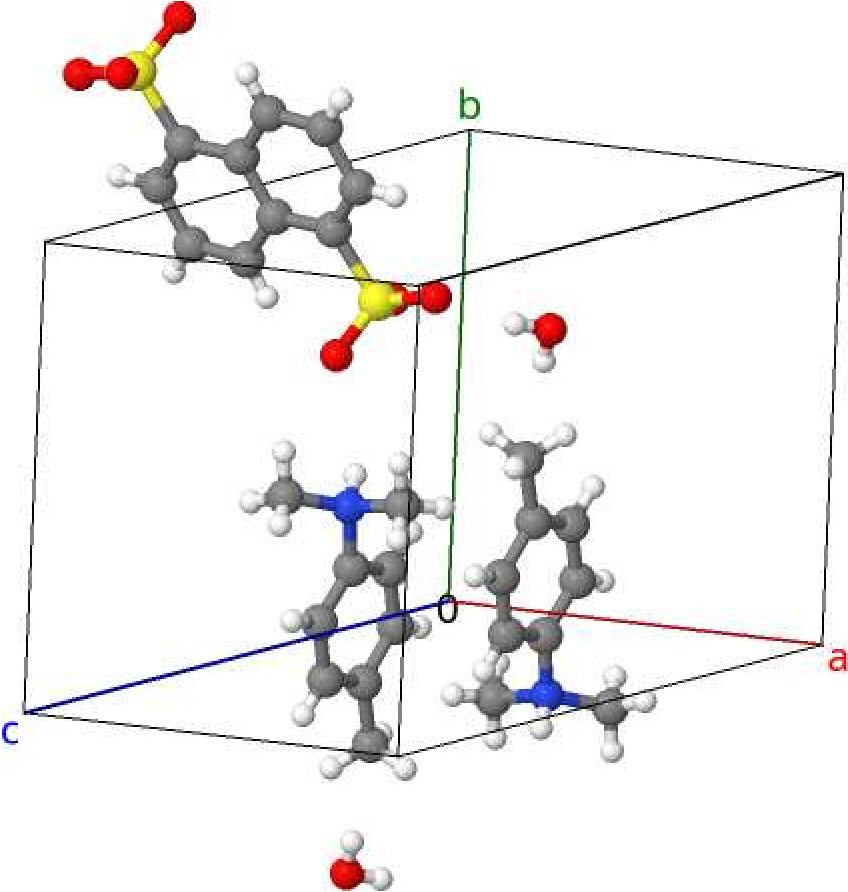
\includegraphics[scale=0.20]{pictures/2231955-chemical}};
    \node at (7,-2) {\small\itshape Stoichiometrically correct molecule};
\end{tikzpicture}

There are special kind of molecules, \textit{polymeric} molecules. Technical term is \textit{coordination polymers}, and there is a long history of problems with definitions \cite{Batten1998, Batten2012, Batten2013}. For our purposes we will consider \textit{polymer} an infinite molecule, which can be represented by an infinite repeated net. Infinite nature of \textit{polymers} presents problem on how to create a finite representation of such molecule.
There is an algorithm\cite{Chung1984} to solve this problem. It uses \textit{quotient graph} to describe all translational equivalent bonds and atoms. \textit{Quotient graph} algorithm uses notion of \textit{equivalence} to group \textit{equivalent} objects, in our case atoms are \textit{equivalent} if they have the same \textit{label} and \textit{symmetry operation} and algorithm will collect all \textit{equivalent} atoms into groups and add connections (edges) between them, we assign value to the edges.

Algorithm to create \textit{Labeled Quotient Graph} (LQG):

\begin{enumerate}\itemsep0pt
    \item Choose a coordinate system, select basis vectors.
    \item Assign initial labels to the original vertices $(0,0,0)$.
    \item If the net has an edge from point $P(m,n)$ to point $R(p,q)$ $\Rightarrow$ there is a directed edge in \textit{LQG} with label $(p-m, q-n)$ from $P$ to $R$.
\end{enumerate}

\begin{tikzpicture}[node distance=0.5cm, font=\small,>=Stealth]

\node[inner sep=0] (net) at (0,0)
    {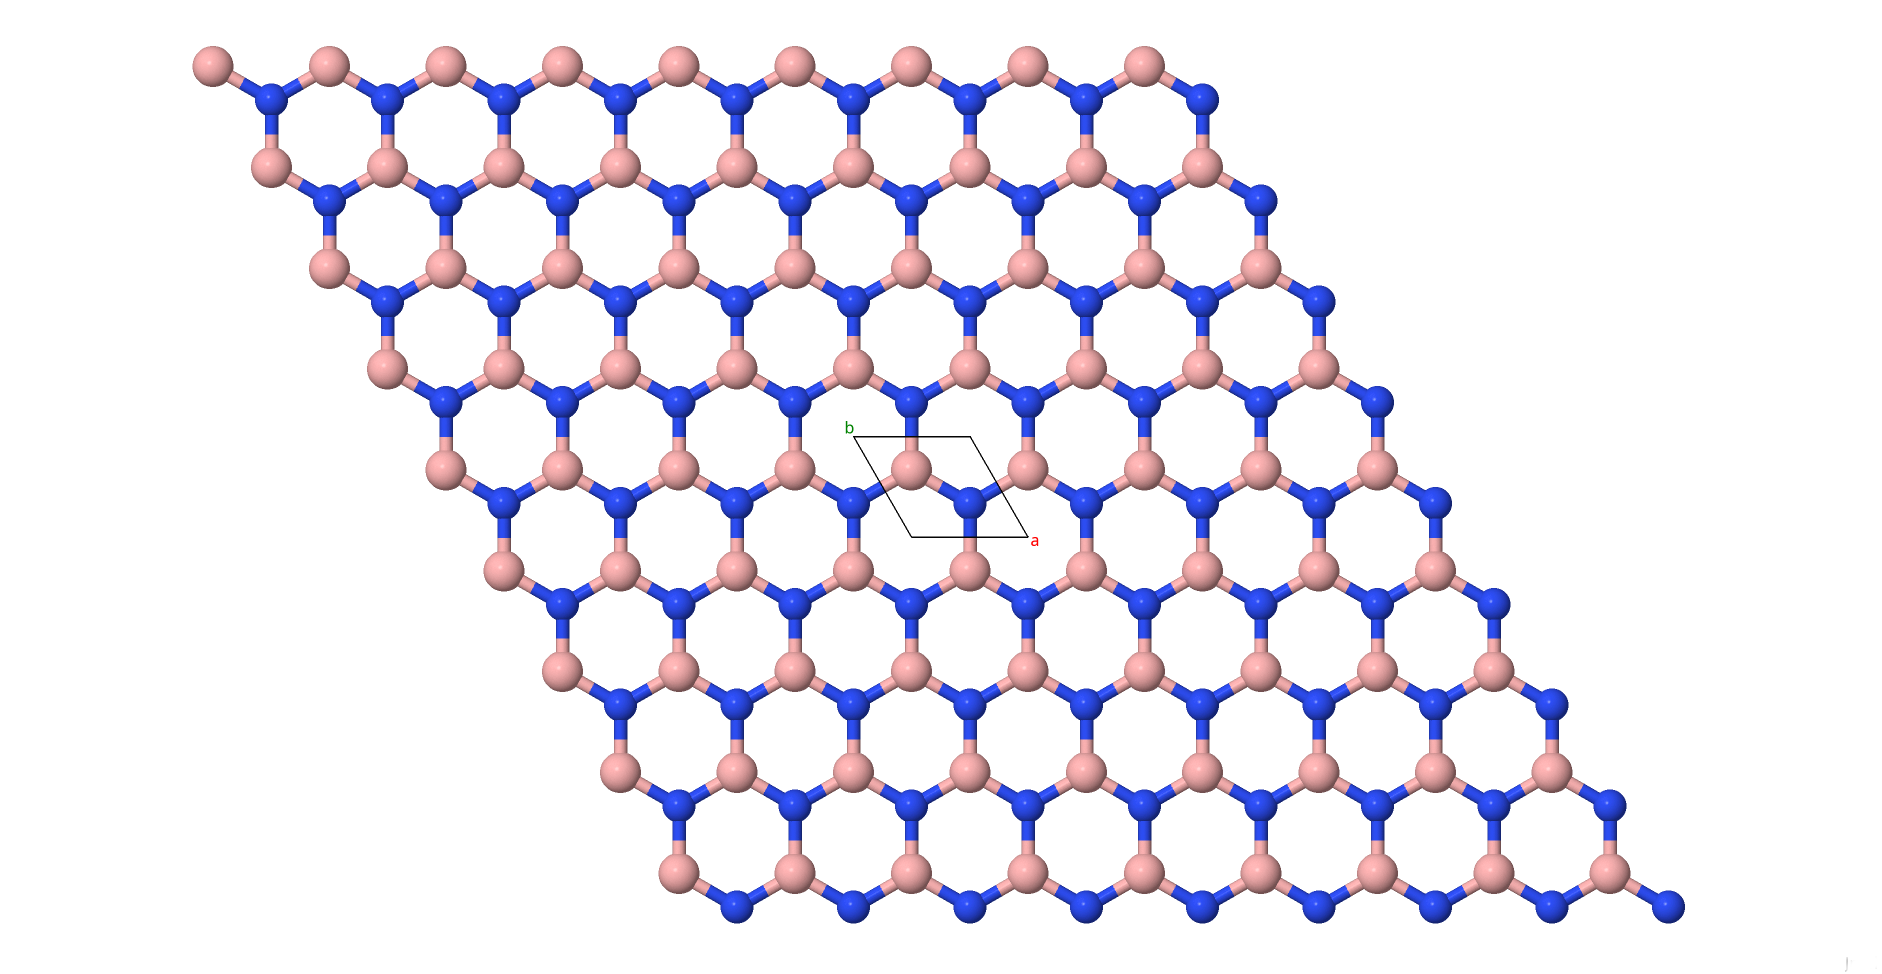
\includegraphics[width=0.4\textwidth]{pictures/9008997_cif_molecule2.png}};
    \node[below=1mm of net.south, font=\scriptsize\itshape] {Infinite net (COD ID \href{http://www.crystallography.net/cod/9008997.html}{\texttt{9008997}})};

\node[inner sep=0, right=5cm of net] (qg)
    {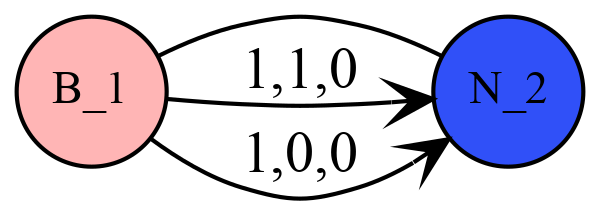
\includegraphics[width=0.25\textwidth]{pictures/9008997qg.png}};
    \node[below=1mm of qg.south, font=\scriptsize\itshape] {Labeled Quotient Graph (COD ID \href{svn://databases.crystallography.lt/quotient-graphs/trunk/outputs/polymers/default/9/00/89/9008997.dot}{\texttt{9008997}})};

\node[inner sep=0, right=3.5cm of net, below=2cm of $(net)!0.5!(qg)$] (tikzgraph){
    \begin{circuitikz}[scale=1]

        \draw (-1,26)--(2,26)--(3.5,24.25)--(0.5,24.25)--cycle;
        \draw (-4,26)--(-1,26)--(0.5,24.25)--(-2.5,24.25)--cycle;
        \draw (-2.5,27.75)--(0.5,27.75)--(2,26)--(-1,26)--cycle;

        \draw[short] (-1,24.75)--(0.5,25.5);
        \draw[short] (0.5,25.5)--(0.5,26.75);
        \draw[short] (0.5,25.5)--(2,24.75);

        \draw[fill={rgb,255:red,48; green,80; blue,248}]
            (0.5,26.75) circle(0.25cm) node[anchor=east, xshift=-10pt, yshift=-1pt, font=\scriptsize]{1,1,0};
        \draw[fill={rgb,255:red,48; green,80; blue,248}]
            (2,24.75) circle(0.25cm) node[anchor=east, xshift=-10pt, yshift=-1pt, font=\scriptsize]{1,0,0};
        \draw[fill={rgb,255:red,255; green,181; blue,181}]
            (0.5,25.5) circle(0.25cm) node[anchor=east, xshift=-10pt, yshift=-1pt, font=\scriptsize]{0,0,0};
        \draw[fill={rgb,255:red,48; green,80; blue,248}]
            (-1,24.75) circle(0.25cm) node[anchor=east, xshift=-10pt, yshift=-1pt, font=\scriptsize]{0,0,0};

        \coordinate(origin) at (-2.5,24.25);
        \coordinate(veca) at (3.5,24.25);
        \coordinate(vecb) at (-4,26);
        \draw[->,thick,red](origin)--(veca) node[midway,below,font=\scriptsize]{$\mathbf{a}$};
        \draw[->,thick,blue](origin)--(vecb) node[midway,left,font=\scriptsize]{$\mathbf{b}$};

    \end{circuitikz}
};
\node[below=1mm of tikzgraph.south, font=\scriptsize\itshape] 
    {Constructing Labeled Quotient Graph (LQG)};

\end{tikzpicture}

On the left you can see \textit{honycomb} net, at the center is a visual representation of the construction of \textit{LQG} and on the right is the result --- \textit{LQG}, vertex \textit{B\_1} represents all the \textit{Boron} atoms with symmetry operation 1, and vertex \textit{N\_2} represents all the \textit{Nitrogen} atoms with symmetry operation 2, 3 edges between these vertices represent all the possible translations that atoms can take, and can be used to reconstruct molecule.

\textit{LQG} algorithm was implemented in \textit{cif\_molecule} and released in \textit{cod-tools} release \textit{3.11.0}\cite{cod-tools}. \textit{cif\_molecule} were used on all the entries in the \textit{Crystallography Open Database} (COD)\cite{Grazulis2011}.

In addition to multiple tests that were already present, number of tests were added to the \textit{cif\_molecule}. But it is impossible to predict all the possible test cases. This potentially makes this algorithm a good target for creating formal specification that can be proved and improve confidence in the algorithm.


\section{Implementation}
The first step is to define all the datatypes and functions in a common module so we can reuse it.
Translation is just a vector that represents atom translation. Atom consist of atom label, \textit{sym} --- symmetry operation, and translation.
Vertex contains just atom label and symmetry operation, which what we use to define \textit{equivalence} for atoms. Function \textit{Id} returns vertex from an atom, and \textit{AllNodeIds} returns all the Ids (vertices) from sequence of atoms using set comprehension.

\begin{lstlisting}[caption={Common module},label={lst:common}]
module Common {
  datatype Translation = Translation(x: int, y: int, z: int)
  datatype Atom   = Atom(atomLabel: string, sym: int,
                         translation: Translation)

  datatype Vertex = Vertex(atomLabel: string, sym: int)
  datatype Bond = Bond(a: Atom, b: Atom)
  datatype Edge = Edge(u: Vertex, v: Vertex,
                       shift: Translation)

  function Id(a: Atom): Vertex { Vertex(a.atomLabel, a.sym) }

  function AllNodeIds(atoms: seq<Atom>): set<Vertex> {
    set i | 0 <= i < |atoms| :: Id(atoms[i])
  }

  function Subtract (u: Translation, v: Translation):
                Translation {
                    Translation(u.x-v.x, u.y-v.y, u.z-v.z)
                }
}
\end{lstlisting}

Now we can implement the algorithm for constructing \textit{LQG}. We need to simplify input and output, method will accept sequences of atoms and bonds, and will return sets of vertices and edges which will represent \textit{LQG}.

\begin{lstlisting}[caption={ConstructLQG specification},label={lst:constructsepcification}, literate={{forall}{forall}6 {exists}{exists}6}]
method ConstructLQG(atoms: seq<Atom>, bonds: seq<Bond>)
returns (V: set<Vertex>, E: set<Edge>)
  requires |atoms| > 0
  requires forall b :: b in bonds ==> b.a in atoms &&
                                    b.b in atoms
  ensures forall e1,e2 | e1 in E && e2 in E && e1 != e2 ::
  !(e1.u == e2.v && e1.v == e2.u &&
    e1.shift == Negate(e2.shift))
  ensures forall i | 0 <= i < |atoms| :: Id(atoms[i]) in V
  ensures V == AllNodeIds(atoms)
\end{lstlisting}

Our only preconditions are that there are atoms, and that they are connected. In postconditions we make sure that all atoms are represented in the vertices, and that no distinct edges are inverses of each other, and that vertices contain all \textit{equivalent} classes from atoms.

We assume that molecule connected and since we already have all the bonds we get all the node ids from atoms, and assign visited. Than iterate over all atoms, add invariant to verify that no opposite edges added.

\begin{lstlisting}[caption={Outer loop},label={lst:invariant1}, literate={{forall}{forall}6 {exists}{exists}6}]
var allNodeIds := AllNodeIds(atoms);
var visited : set<Vertex> := allNodeIds;
var edges : set<Edge> := {};

var atomIdx := 0;
while atomIdx < |atoms|
  decreases |atoms| - atomIdx
  invariant forall e1,e2 | e1 in edges && e2 in edges &&
                                          e1 != e2 ::
    !(e1.u == e2.v && e1.v == e2.u &&
        e1.shift == Negate(e2.shift))
{
\end{lstlisting}

Iterate over all the bonds make sure to not add opposite edge.
\begin{lstlisting}[caption={Inner loop},label={lst:invariant2}, literate={{forall}{forall}6 {exists}{exists}6}]
var currentAtom := atoms[atomIdx];
atomIdx := atomIdx + 1;
var currentNodeId := Id(currentAtom);

var bondIdx := 0;
while bondIdx < |bonds|
  decreases |bonds| - bondIdx
  invariant forall e1,e2 | e1 in edges && e2 in edges &&
                                          e1 != e2 ::
  !(e1.u == e2.v && e1.v == e2.u &&
        e1.shift == Negate(e2.shift))
{
\end{lstlisting}

Only process bonds that have current atom, if bond contains current atom calculate edge label, and if this edge has not been added yet, add it to the set.
\begin{lstlisting}[caption={Inner loop, body},label={lst:invariant2}]
var bond := bonds[bondIdx];
bondIdx := bondIdx + 1;

if bond.a == currentAtom {
  var neighborNodeId := Id(bond.b);
  var shift := Subtract(bond.b.translation,
                        bond.a.translation);
  var edge := Edge(currentNodeId, neighborNodeId, shift);
  var invEdge := Edge(neighborNodeId,
                      currentNodeId,
                      Negate(shift));

  if edge !in edges && invEdge !in edges {
    edges := edges + {edge};
  }
} else if bond.b == currentAtom {
\end{lstlisting}

Text\_Construct module were created in order to test construction of the \textit{LQG}. There we construct molecule that we seen in~\ref{sec:description}, we add minimal number of atoms and bonds needed to construct \textit{LQG}. After constructing \textit{LQG} auxiliary lemma called to prove number of vertices and that they are in the set.

\begin{lstlisting}[caption={Test construction of \textit{LQG} from molecule},label={lst:molecule}]
var B0 := Atom("B",1, Translation(0,0,0));
var N00 := Atom("N",2, Translation(0,0,0));
var N10 := Atom("N",2, Translation(1,0,0));
var N11 := Atom("N",2, Translation(1,1,0));

var atoms := [B0, N00, N10, N11];
var bonds := [Bond(B0,N00), Bond(B0,N10), Bond(B0,N11)];

var V, E := ConstructLQG(atoms, bonds);
...

TestCaseNodeIdProperties(atoms);
assert |V| == 2;
assert Vertex("B", 1) in V;
assert Vertex("N", 2) in V;
\end{lstlisting}

Since it is in the Main method, when compiled this code will print results.

\begin{verbatim}
Results:
|V| = 2 unique vertices
|E| = 3 edges
Test 0 vertex Common.Vertex.Vertex("B", 1)
Test 1 vertex Common.Vertex.Vertex("N", 2)
Vertex count: 2
Test 0 edge Common.Edge.Edge(Common.Vertex.Vertex("B", 1),
                             Common.Vertex.Vertex("N", 2),
                             Common.Translation.Translation(0, 0, 0))
Test 1 edge Common.Edge.Edge(Common.Vertex.Vertex("B", 1),
                             Common.Vertex.Vertex("N", 2),
                             Common.Translation.Translation(1, 0, 0))
Test 2 edge Common.Edge.Edge(Common.Vertex.Vertex("B", 1),
                             Common.Vertex.Vertex("N", 2),
                             Common.Translation.Translation(1, 1, 0))
Edges count: 3
\end{verbatim}

Dafny version \textit{4.10.1} was used for executions. Program were split into modules, and executed using \textit{make}. Default target will run \textit{verify} command with option \texttt{--log-format text} and results of the execution will be stored in the \texttt{results/verification/verify.log}. Target \textit{build} will run \textit{build} command, build log will be stored in the \texttt{results/build/build.log}, directory \texttt{results/build/} will store executables.


\section{Conclusions}
Dafny is a powerful language and a automated program verifier with rich set of features. Unfortunately only simplified version of the algorithm was implemented, and proof is rudimentary. It is hard to come up with a proper postconditions and the proof. Additional method to reconstruct molecule from \textit{LQG} was implemented but it is very simplified, and does not follows the original algorithm.
After more practice and exposure to formal methods I think I will be able to improve my implementation.


\bibliographystyle{plain}
\bibliography{./bibliography/citations}

\end{document}
